\documentclass{article}
\usepackage[utf8]{inputenc}
\usepackage[spanish]{babel}

\usepackage{graphicx} % Required for inserting images
\usepackage{imakeidx}
\usepackage{amssymb, amsmath}
\usepackage{listings}
\usepackage{xcolor}
\usepackage{hyperref}
\makeindex
\setlength{\parindent}{12pt}

\definecolor{darkgreen}{RGB}{0, 150, 0}

% Para poner código de python en el documento
\lstdefinestyle{mystyle}{
  backgroundcolor=\color{white},
  commentstyle=\color{darkgreen},
  keywordstyle=\color{blue},
  numberstyle=\tiny\color{gray},
  stringstyle=\color{red},
  basicstyle=\ttfamily,
  breaklines=true,
  numbers=left,
  numbersep=5pt,
  showstringspaces=false,
  language=Python
}


% Márgenes de página
\usepackage[left=2.5cm, right=2.5cm, top=3cm, bottom=3cm]{geometry}

% Fuente y formato
\usepackage[T1]{fontenc} % Para las ñ y letras con tilde
\usepackage{times}
\usepackage{microtype} % Mejora el espaciado de las palabras

% Encabezado y pie de página
\usepackage{fancyhdr}
\pagestyle{fancy}
\fancyhf{} % Borra el encabezado y pie de página existentes
\rhead{Rubén Nogueras González \& Pelayo Huerta Mijares}
\rfoot{\thepage}


\begin{document}
    \begin{titlepage}
    \centering
    {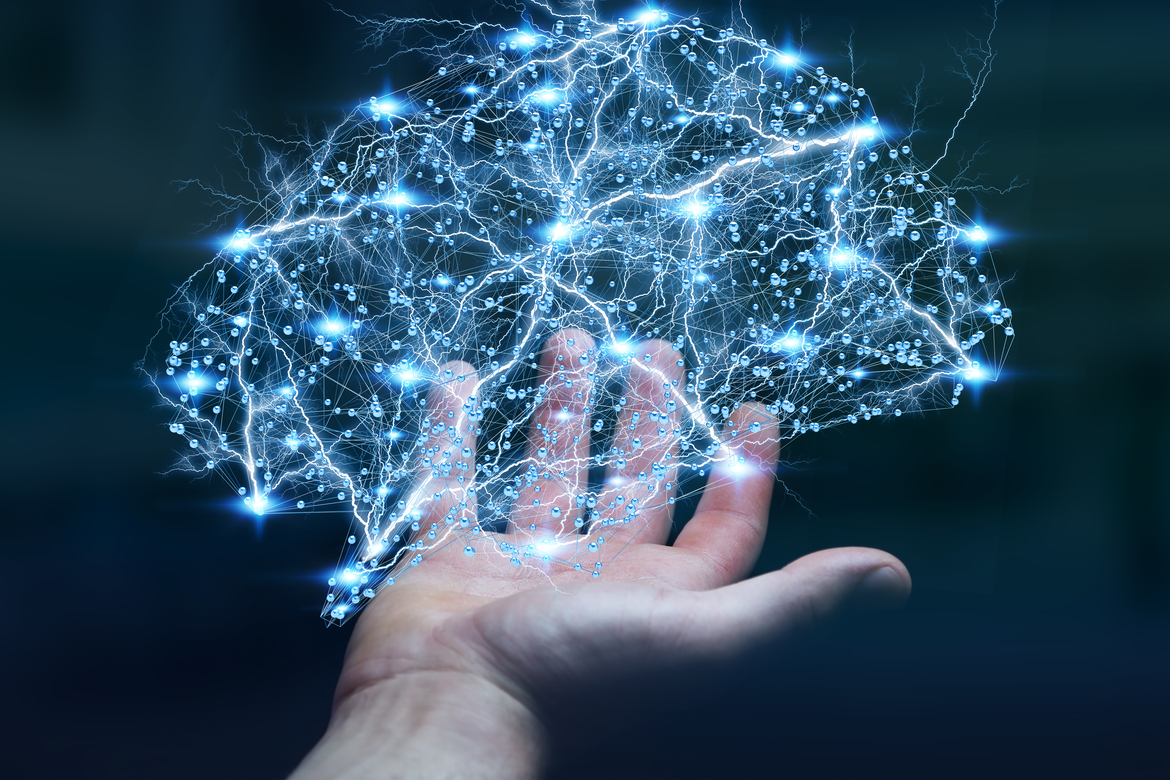
\includegraphics[width=0.8\textwidth]{portada.png}\par}
    \vspace{1cm}
    {\bfseries\LARGE Universidad Alfonso X \par}
    \vspace{3cm}
    {\scshape\Huge Técnicas de Optimización y Control \par}
    \vspace{2cm}
    {\itshape\Large Práctica 11 \par}
    \vspace{1cm}
    {\Large Autores: \par}
    {\Large Pelayo Huerta Mijares \par}
    {\Large Rubén Nogueras González \par}
    \vfill
    {\Large Noviembre 2023 \par}
    \end{titlepage}


\section{Redes de Atención Gráfica (GAT)}

\subsection{Atención en Redes Neuronales}

Antes de profundizar en las GAT, es importante entender el concepto de atención en las redes neuronales. La atención es un mecanismo que permite a la red dar más peso a ciertas partes de la entrada en función de su relevancia para la tarea en cuestión. Las redes de atención son útiles para procesar secuencias y seleccionar partes importantes de ellas.

\subsection{Redes de Atención Gráfica (GAT)}

Las GAT aplican la idea de atención a los grafos. En lugar de tratar todos los nodos por igual, las GAT asignan pesos de atención a los nodos vecinos en función de su importancia relativa para el nodo central. Cada nodo en una GAT calcula un conjunto de pesos de atención para sus nodos vecinos utilizando una función de atención. Estos pesos se utilizan para combinar las representaciones de los nodos vecinos en una representación agregada para el nodo central. La fórmula típica para calcular los pesos de atención en una GAT es mediante una operación de atención basada en redes neuronales (por ejemplo, una red neuronal feedforward). Esta operación asigna pesos a los nodos vecinos en función de sus características y las del nodo central. Los pesos de atención pueden ser normalizados utilizando funciones de activación como la función Softmax para que sumen 1, lo que garantiza que se distribuya la atención correctamente.

\subsection{Capas Múltiples}

Las GAT pueden tener varias capas, lo que permite realizar múltiples pasos de atención. Esto ayuda a capturar patrones de relaciones más complejos en los grafos.

\subsection{Aplicaciones}

Las GAT se utilizan en una variedad de aplicaciones, como la recomendación de redes sociales, el procesamiento del lenguaje natural, la bioinformática y la detección de anomalías en redes, entre otras.

\vspace{1cm}

\section{Capa de atencion}

\vspace{1cm}

En esta sección vamos a explicar más detalladamente la capa de atención (mencionada anteriormente) de una Red de Atención Gráfica (GAT).

\vspace{0.5cm}

La autotención permite que un nodo en un grafo considere la información de sus nodos vecinos, asignando pesos a esos vecinos en función de su importancia relativa para el nodo central. En otras palabras, algunos nodos tienen mayor importancia.

\vspace{0.5cm}

Cabe destacar que hablamos de autoatención y no de atención ya que las entradas de los nodos se comparan entre sí.

\vspace{0.5cm}

Cada nodo en un grafo, denotado como 'i', posee un vector de características 'Xi' que describe sus atributos o información específica. La capa de Red de Atención Gráfica (GAT) calcula la representación actualizada del nodo 'i' al combinar información de sus vecinos en el grafo. Esta combinación se logra mediante el cálculo de un conjunto de coeficientes de atención que ponderan las características de los nodos vecinos, y luego se multiplican por una matriz de pesos compartida 'W'.

\vspace{0.5cm}

\begin{equation}
    h_{i} = \alpha_{11}Wx_{1} + \alpha_{12}Wx_{2} + \alpha_{13}Wx_{3} + \alpha_{14}Wx_{4}
\end{equation}

\vspace{0.5cm}

Y para calcular dichos coeficientes de atención, podemos obtener sus valores mediante una red neuronal. Destacamos 4 pasos:

\vspace{1cm}

\subsection{Transformación Lineal}

\vspace{1cm}

Concatenamos vectores de atributos de un pares de nodos, por lo que podemos aplicar una transformación lineal, con una matriz de peso correspondiente $W_{att}$.

\vspace{0.5cm}

\begin{equation}
    a_{ij} = W_{att}^{t} [Wx_{i} || Wx_{j}]
\end{equation}

\vspace{0.5cm}

\begin{center}
    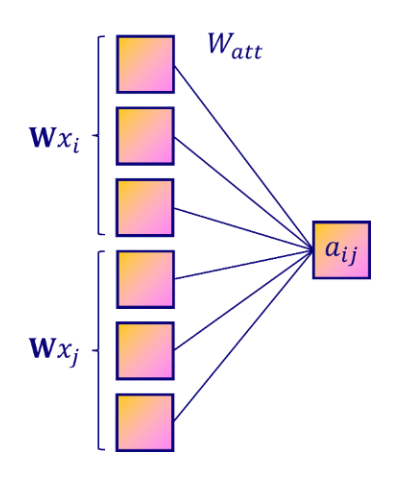
\includegraphics[width=0.5\linewidth]{Watt.png}
\end{center}

\vspace{1cm}

\subsection{Función de activación}

\vspace{1cm}

Integramos no linealidad, ya que estamos con una red neuronal, y esto lo hacemos mediante una función de activación (elegimos la función LeakyReLU).

\vspace{0.5cm}

\begin{equation}
    e_{ij} = LeakyReLU(a_{ij})
\end{equation}

\vspace{0.5cm}

\begin{center}
    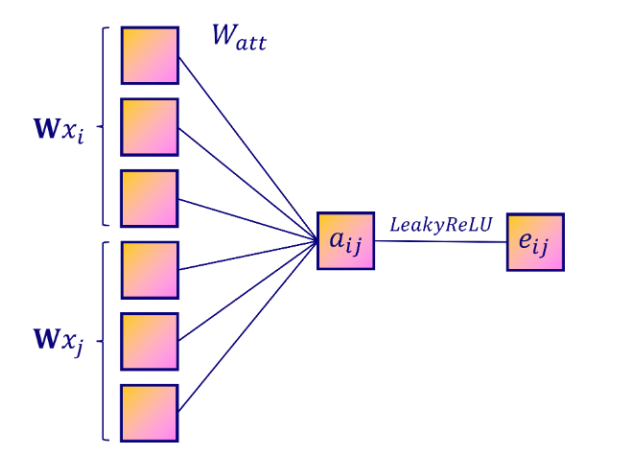
\includegraphics[width=0.75\linewidth]{foto2.png}
\end{center}

\vspace{1cm}

\subsection{Normalización Softmax}

\vspace{1cm}

Hay un problema, y es que la salida de dicha red neuronal no está normalizada, ya que queremos comparar los coeficientes. Por lo tanto aplicamos la función softmax a todos los nodos vecinos:

\vspace{0.5cm}

\begin{equation}
    \alpha_{ij} = softmax_{j}(e_{ij}) = \frac{exp(e_{ij})}{\sum_{k \in N_{i}}exp(e_{ik})}
\end{equation}

\vspace{0.5cm}

\begin{center}
    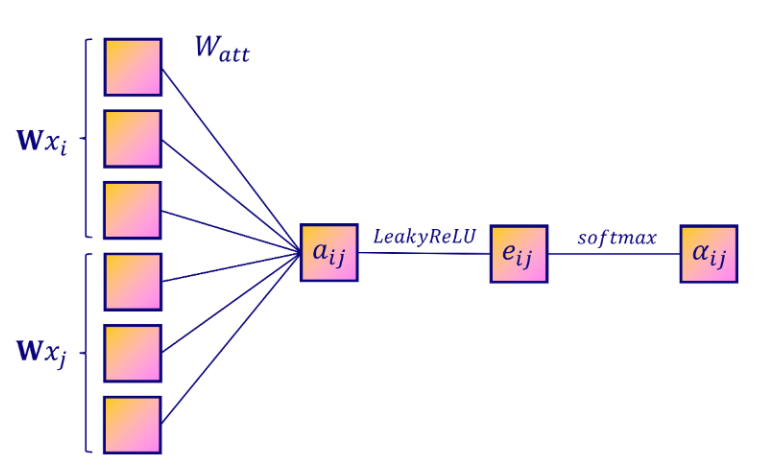
\includegraphics[width=0.75\linewidth]{softmax.png}
\end{center}

\vspace{1cm}

\subsection{Atención de múltiples cabezas}

\vspace{1cm}

Con softmax, ya tenemos los coeficientes de atención, el último problema qu se nos presenta es que la autoatención no es muy estable, y para solucionar esto, introducimos la atención de múltiples cabezas en la arquitectura del transformador.

\vspace{0.5cm}

Dichos transformadores, son un caso particular de GNN, de ahí su similitud, y gracias a ellos podemos incluir la atención de varias cabezas (una idea del procesamiento del lenguaje natural).

\vspace{0.5cm}

\begin{center}
    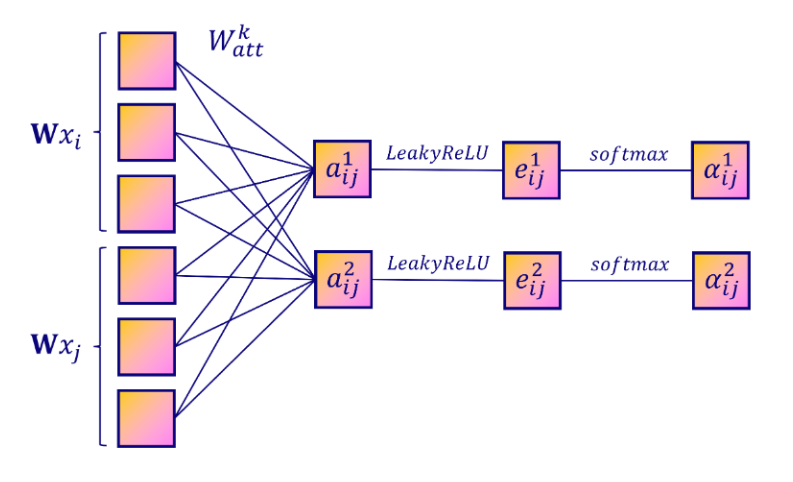
\includegraphics[width=0.75\linewidth]{transformadores.png}
\end{center}

\vspace{0.5cm}

En los GAT, en el proceso de atención multicabezal se repiten los mismos 3 pasos para hacer un promedio o concatenar los resultados:

\vspace{0.5cm}

\begin{itemize}
    \item \textbf{Promedio}: 
        \begin{equation}
            h_{i} = \frac{1}{n} \sum_{k=1}^{n} h_{i}^{k}
        \end{equation}
    \item \textbf{Concatenación}:
        \begin{equation}
             h_{i} = ||_{k=1}^{n}h_{i}^{k}
        \end{equation}
\end{itemize}

\vspace{0.5cm}

En la implementación práctica, empleamos el método de concatenación cuando se trata de una capa oculta, mientras que utilizamos el enfoque de promedio cuando se trata de la capa final (de salida). En la mayoría de los casos, apilamos múltiples capas GAT para incluir un vecindario más extenso, lo que nos permite combinar estos dos enfoques dentro del mismo modelo GAT.

\vspace{1cm}

\section{Implementando una Red de Atención Gráfica}

\vspace{1cm}

En este apartado implementaremos un GAT en Python usando PyTorch Geometric usando la capa Gatv2Conv.

\vspace{0.5cm}

\begin{lstlisting}[style=mystyle]
import torch.nn.functional as F
from torch.nn import Linear, Dropout
from torch_geometric.nn import GCNConv, GATv2Conv

class GCN(torch.nn.Module):
    """Graph Convolutional Network"""
    def __init__(self, dim_in, dim_h, dim_out):
      super().__init__()
      self.gcn1 = GCNConv(dim_in, dim_h)
      self.gcn2 = GCNConv(dim_h, dim_out)
      self.optimizer = torch.optim.Adam(self.parameters(),
                                        lr=0.01,
                                        weight_decay=5e-4)
    def forward(self, x, edge_index):
        h = F.dropout(x, p=0.5, training=self.training)
        h = self.gcn1(h, edge_index).relu()
        h = F.dropout(h, p=0.5, training=self.training)
        h = self.gcn2(h, edge_index)
        return h, F.log_softmax(h, dim=1)

class GAT(torch.nn.Module):
    """Graph Attention Network"""
    def __init__(self, dim_in, dim_h, dim_out, heads=8):
        super().__init__()
        self.gat1 = GATv2Conv(dim_in, dim_h, heads=heads)
        self.gat2 = GATv2Conv(dim_h*heads, dim_out, heads=1)
        self.optimizer = torch.optim.Adam(self.parameters(),
                                          lr=0.005,
                                          weight_decay=5e-4)

    def forward(self, x, edge_index):
        h = F.dropout(x, p=0.6, training=self.training)
        h = self.gat1(h, edge_index)
        h = F.elu(h)
        h = F.dropout(h, p=0.6, training=self.training)
        h = self.gat2(h, edge_index)
        return h, F.log_softmax(h, dim=1)

def accuracy(pred_y, y):
    """Calculate accuracy."""
    return ((pred_y == y).sum() / len(y)).item()

def train(model, data):
    """Train a GNN model and return the trained model."""
    criterion = torch.nn.CrossEntropyLoss()
    optimizer = model.optimizer
    epochs = 200
    model.train()
    for epoch in range(epochs+1):
        # Training
        optimizer.zero_grad()
        _, out = model(data.x, data.edge_index)
        loss = criterion(out[data.train_mask], data.y[data.train_mask])
        acc = accuracy(out[data.train_mask].argmax(dim=1), data.y[data.train_mask])
        loss.backward()
        optimizer.step()
        # Validation
        val_loss = criterion(out[data.val_mask], data.y[data.val_mask])
        val_acc = accuracy(out[data.val_mask].argmax(dim=1), data.y[data.val_mask])
        # Print metrics every 10 epochs
        if(epoch % 10 == 0):
            print(f'Epoch {epoch:>3} | Train Loss: {loss:.3f} | Train Acc: '
                  f'{acc*100:>6.2f}% | Val Loss: {val_loss:.2f} | '
                  f'Val Acc: {val_acc*100:.2f}%')      
    return model

@torch.no_grad()
def test(model, data):
    """Evaluate the model on test set and print the accuracy score."""
    model.eval()
    _, out = model(data.x, data.edge_index)
    acc = accuracy(out.argmax(dim=1)[data.test_mask], data.y[data.test_mask])
    return acc
%%time
# Create GCN model
gcn = GCN(dataset.num_features, 16, dataset.num_classes)
print(gcn)

# Train and test
train(gcn, data)
acc = test(gcn, data)
print(f'\nGCN test accuracy: {acc*100:.2f}%\n')
\end{lstlisting}

\vspace{0.5cm}

\begin{center}
    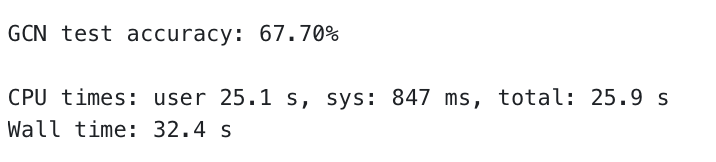
\includegraphics[width=0.5\linewidth]{img/precisionnoentrenado.png}
\end{center}

\vspace{0.5cm}

\begin{center}
    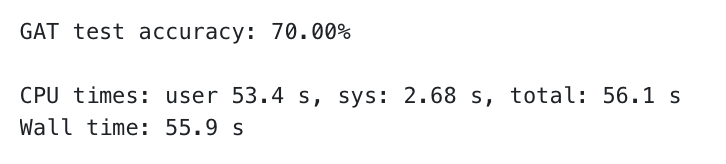
\includegraphics[width=0.5\linewidth]{img/precisionentrenado.png}
\end{center}

\vspace{0.5cm}

En este ejemplo, que a pesar de que no es super riguroso, podemos ver que GAT obtiene una mayor precisión (70,0\%) que GCN (67,7\%). Sin embargo, GAT tarda 55,9 segundos en entrenarse y GCN tan solo 32,4 segundos. Esto es una compensación que puede causar problemas de escalabilidad cuando se trabaja con gráficos grandes.

Veamos lo que realmente aprendió el GAT. Esto podemos visualizarlo con el diagrama t-SNE un método poderoso para representar datos de alta dimensión en 2D o 3D. Primero veamos como se veían las incrustaciones antes del entrenamiento:

\vspace{0.5cm}

\begin{lstlisting}[style=mystyle]
# Initialize new untrained model
untrained_gat = GAT(dataset.num_features, 8, dataset.num_classes)

# Get embeddings
h, _ = untrained_gat(data.x, data.edge_index)

# Train TSNE
tsne = TSNE(n_components=2, learning_rate='auto',
         init='pca').fit_transform(h.detach())

# Plot TSNE
plt.figure(figsize=(10, 10))
plt.axis('off')
plt.scatter(tsne[:, 0], tsne[:, 1], s=50, c=data.y)
plt.show()
\end{lstlisting}

\vspace{0.5cm}

\begin{center}
    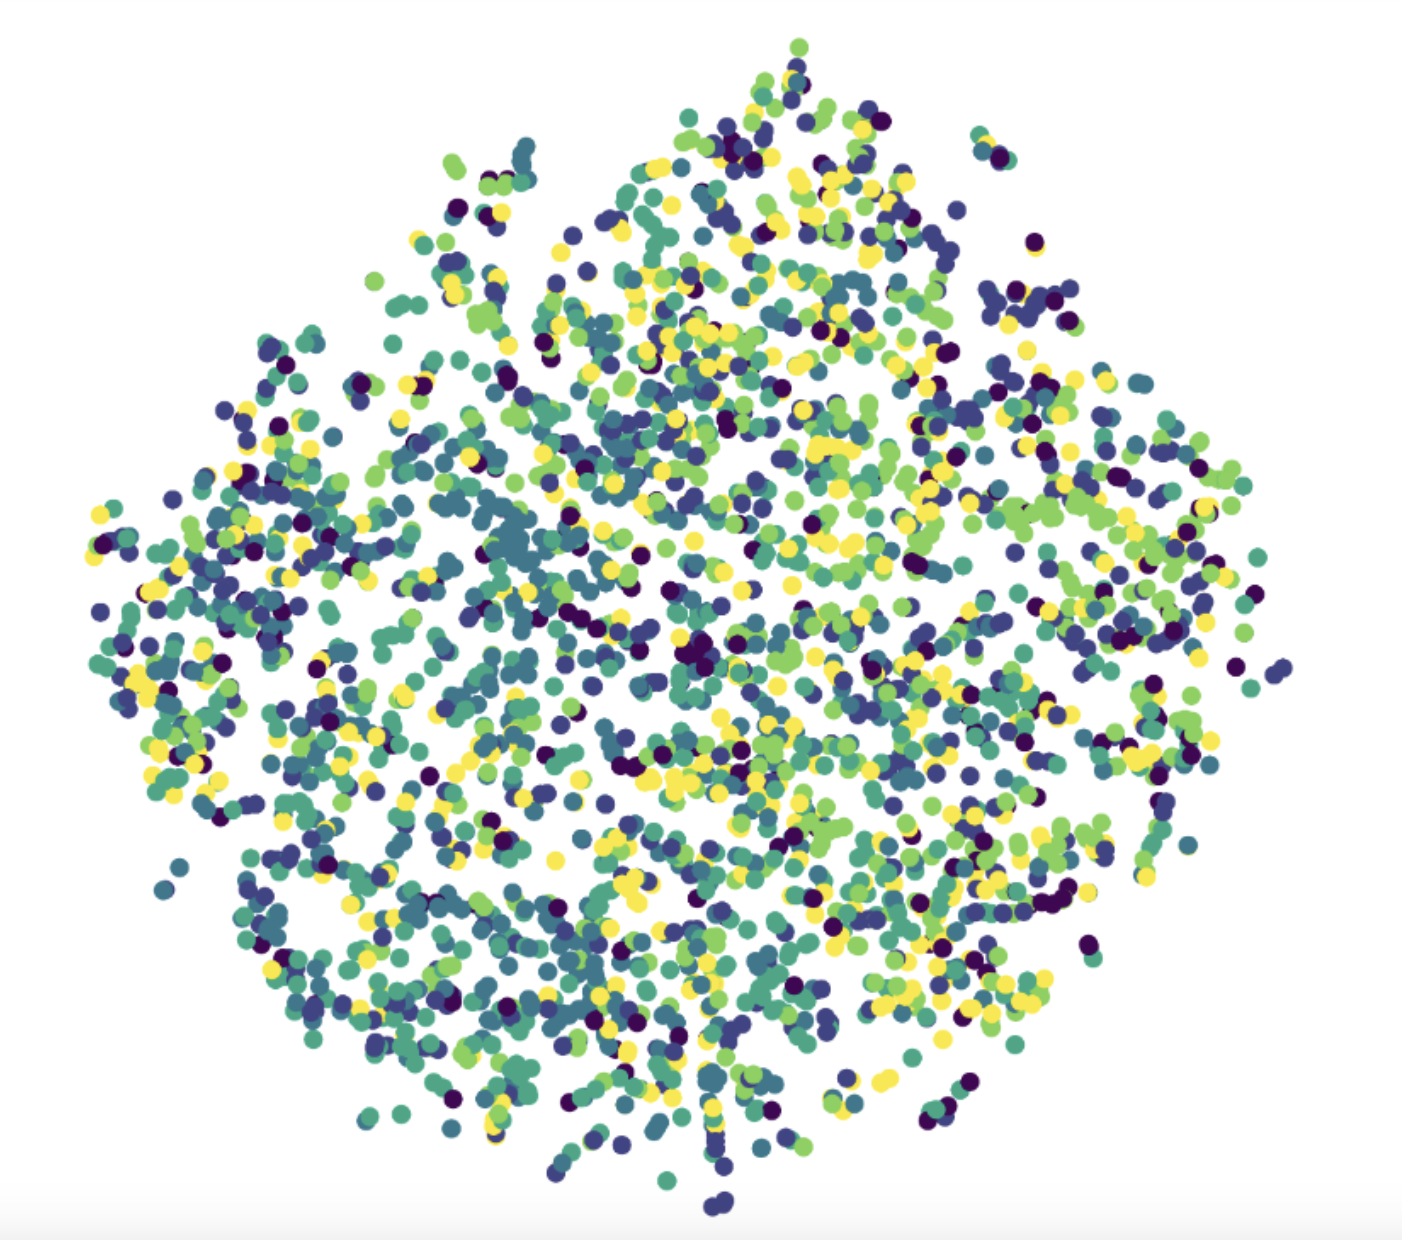
\includegraphics[width=0.75\linewidth]{img/noentrenado.png}
\end{center}

\vspace{0.5cm}

Ahora veamos como se ven las incrustaciones con el modelo entrenado:

\vspace{0.5cm}

\begin{lstlisting}[style=mystyle]
# Get embeddings
h, _ = gat(data.x, data.edge_index)

# Train TSNE
tsne = TSNE(n_components=2, learning_rate='auto',
         init='pca').fit_transform(h.detach())

# Plot TSNE
plt.figure(figsize=(10, 10))plt.axis('off')
plt.scatter(tsne[:, 0], tsne[:, 1], s=50, c=data.y)
plt.show()
\end{lstlisting}

\vspace{0.5cm}

\begin{center}
    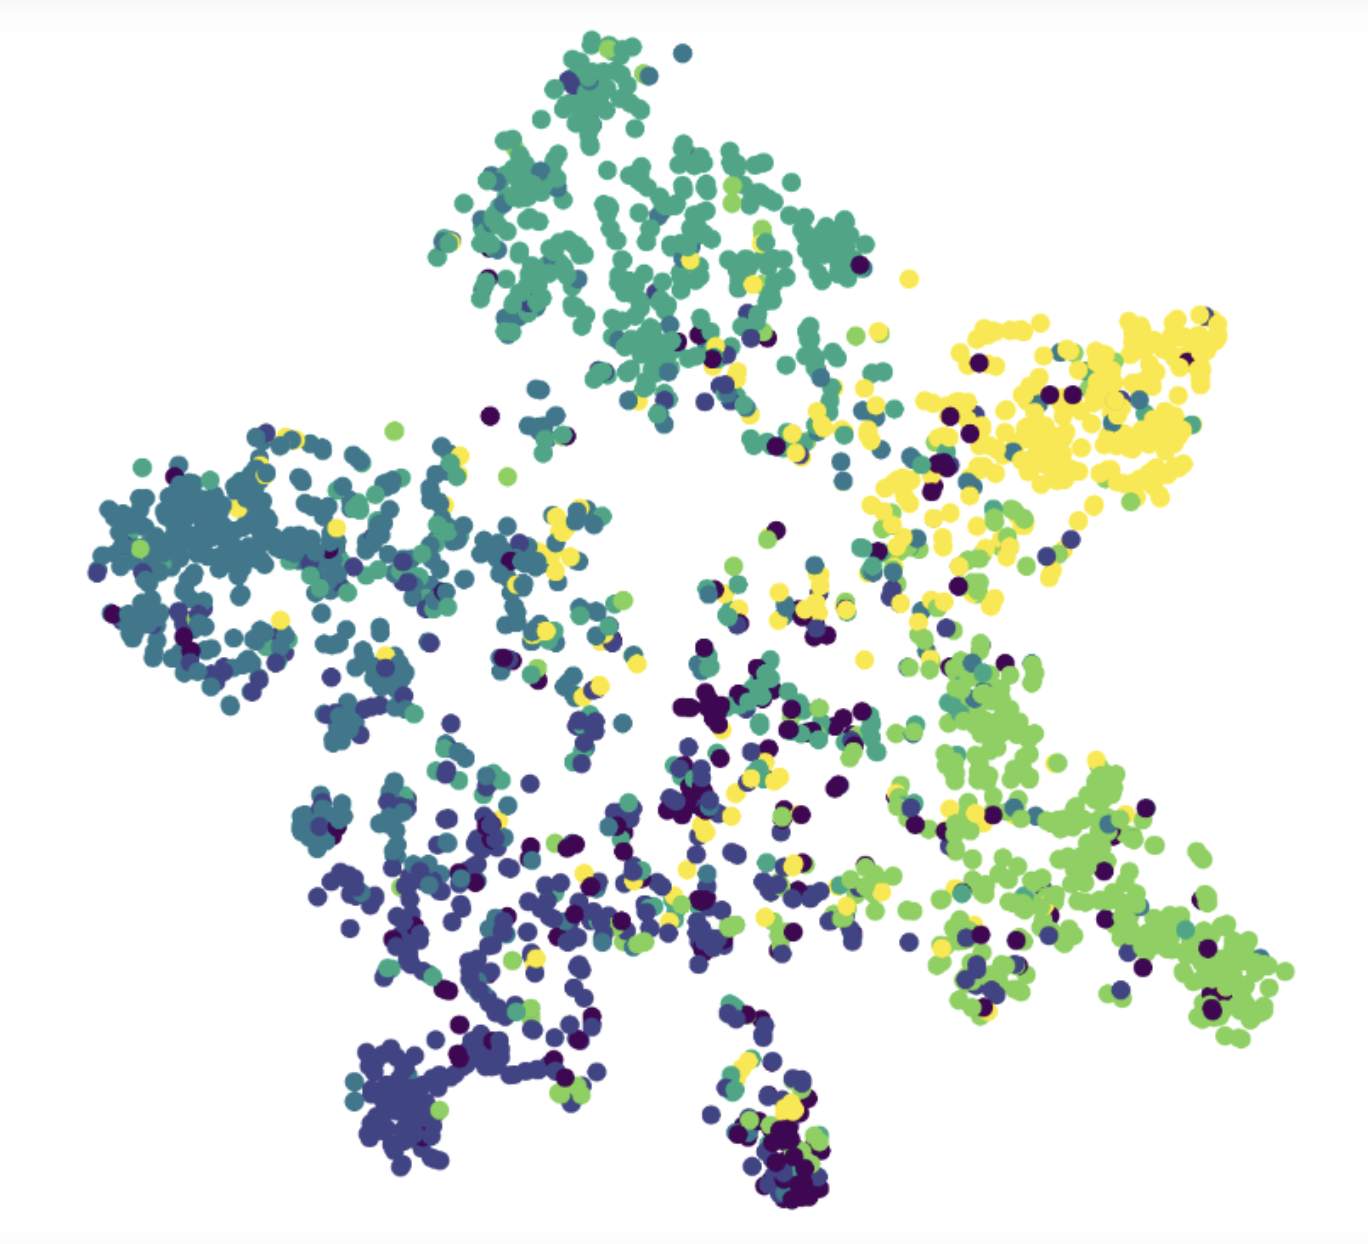
\includegraphics[width=0.75\linewidth]{img/entrenado.png}
\end{center}

\vspace{0.5cm}

Se ven algunas diferencias: en el modelo entrenado vemos como los nodos que pretenecen a las mismas clases, se agrupan. Mientras que en el gráfico del modelo no entrenado, no se ve relación de ningún tipo.
En esta última imagen, podemos ver seis grupos, que corresponden a las seis clases de documentos. También hay valores atípicos, pero es normal ya que nuestra precisión no es perfecta.
Verifiquemos que los nodos mal conectados tengan un impacto negativo en el rendimiento de CiteSeer, calculando la precisión del modelo para cada grado:

\vspace{0.5cm}

\begin{lstlisting}[style=mystyle]
from torch_geometric.utils import degree

# Get model's classifications
_, out = gat(data.x, data.edge_index)

# Calculate the degree of each node
degrees = degree(data.edge_index[0]).numpy()

# Store accuracy scores and sample sizes
accuracies = []
sizes = []

# Accuracy for degrees between 0 and 5
for i in range(0, 6):
  mask = np.where(degrees == i)[0]  
  accuracies.append(accuracy(out.argmax(dim=1)[mask], data.y[mask]))
  sizes.append(len(mask))

# Accuracy for degrees > 5
mask = np.where(degrees > 5)[0]
accuracies.append(accuracy(out.argmax(dim=1)[mask], data.y[mask]))
sizes.append(len(mask))

# Bar plot
fig, ax = plt.subplots(figsize=(18, 9))
ax.set_xlabel('Node degree')
ax.set_ylabel('Accuracy score')
ax.set_facecolor('#EFEEEA')
plt.bar(['0','1','2','3','4','5','>5'],
        accuracies,
        color='#0A047A')
for i in range(0, 7):
    plt.text(i, accuracies[i], f'{accuracies[i]*100:.2f}%',
             ha='center', color='#0A047A')for i in range(0, 7):
    plt.text(i, accuracies[i]//2, sizes[i],
             ha='center', color='white')
\end{lstlisting}

\vspace{0.5cm}

\begin{center}
    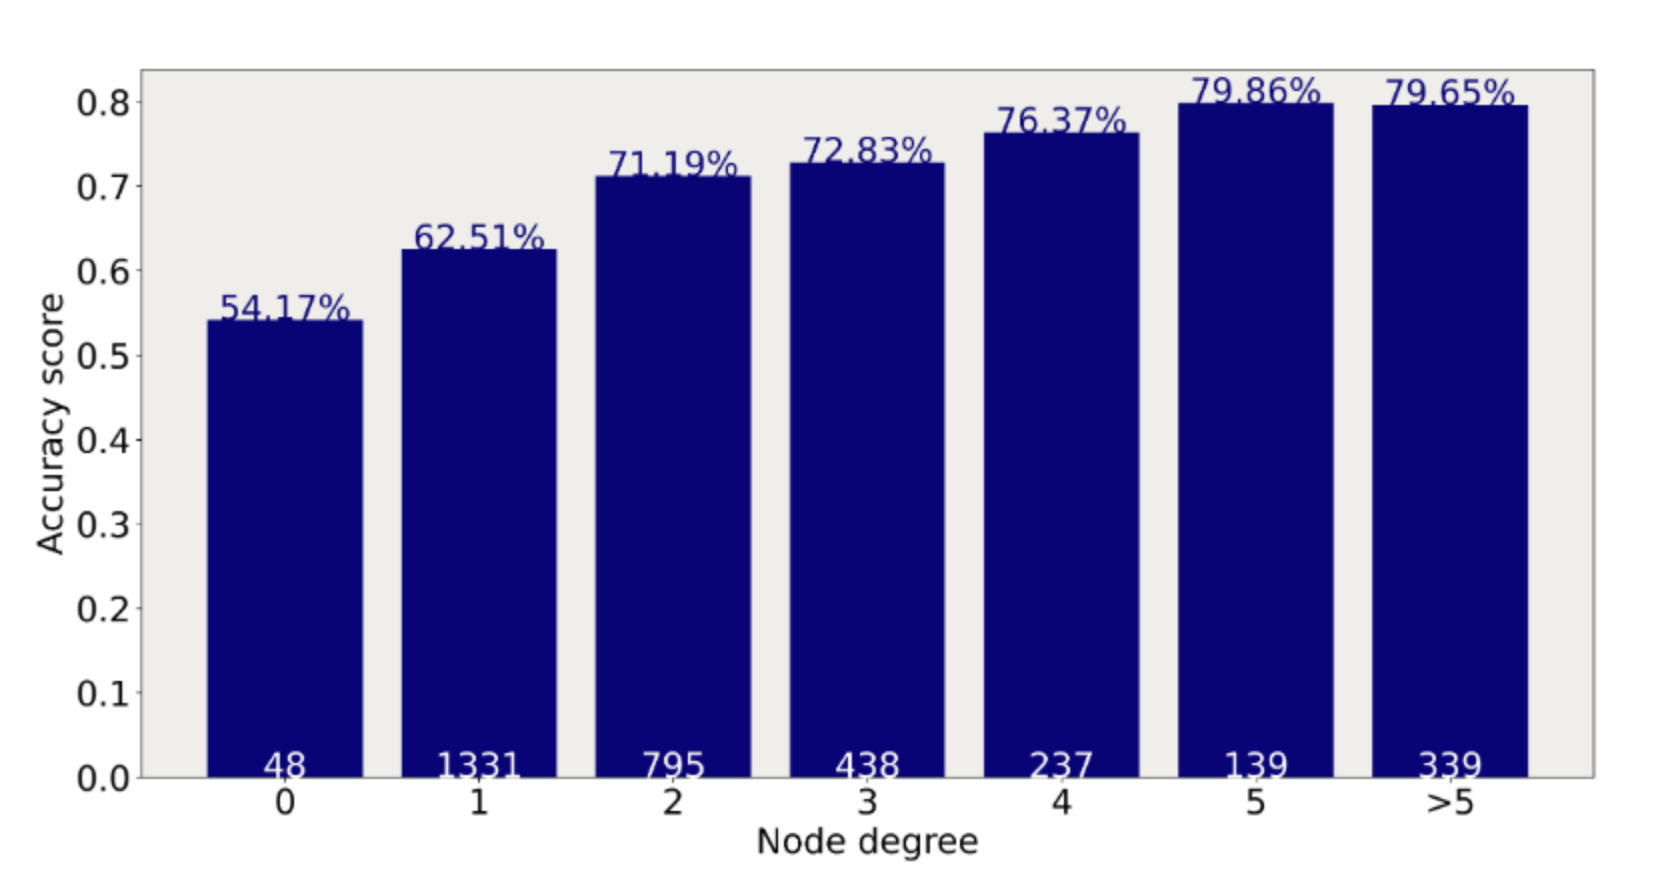
\includegraphics[width=0.75\linewidth]{img/barras.png}
\end{center}

\vspace{0.5cm}

Estos resultados confirman que los nodos con pocos vecinos son más difíciles de clasificar. Cuantas más conexiones relevantes tenga más información podrá agregar.

\vspace{0.5cm}

\section{Conclusión y generalidaz}

\vspace{1cm}

Los Grafos de Autoatención (GAT) han emergido como una herramienta sumamente importante en múltiples contextos, desempeñando un papel crucial en una amplia gama de aplicaciones. Su capacidad para modelar relaciones no lineales entre elementos en conjuntos de datos commplejos, los hacen especialmente poderosos en campos como la inteligencia artificial (IA), ciencia de datos y el procesamiento del lenguaje natural.

En el ámbito de la inteligencia artificial, los GAT han revolucionado la forma en que abordamos problemas de aprendizaje automatico. al permitir la captura de relaciones entre entidades en datos estructurados y no estructurados. Su capacidad para aprender representaciones jerárquicas de datos y reconoces patrones complejos es invaluable en tareas que van desde la recomendación personalizada hasta la visión por computadora.

En el procesamiento del leguaje natural, los GAT se han convertido en un componente fundamental en el análisis y la comprensión de textos. Su capacidad para capturar la semántica y la relación entre palabras y oraciones permite un procesamiento más preciso y contextual mejorando la comprensión del lenguaje natural en sistemas de traducción automática, resumen de texto y análisis de sentimiento.

Por último, en el ámbito de las ciencias biológicas, los GAT se han aplicado con éxito en el análisis de redes moleculares y biológicas, lo que permite entender mejor las interacciones complejas entre diferentes moléculas y proteínas. Esto tiene implicaciones muy significativas en la investigación farmacéutica, el descubrimiento de medicamentos y la comprensión de enfermedade.

La versatilidad de los grafos de automatención (GAT) ha demostrado ser una herramienta de gran relevancia en diversos campos, desde la intelingecia artificial hasta la biología. Su capacidad para modelar relaciones complejas entre entidades lo posiciona como un pilar en la resolución de problemas que involucran datos estructurados y no estructurados, y su continua evolución promete avances significativos en numerosos dominios.

\end{document}
